% !TEX root = ../main.tex < 20 pages
\chapter{Les services web: Vue d'ensemble}
\section{Introduction}
Ce chapitre établit une étude du fondement théorique de notre travail
à savoir les concepts de base du paradigme service Web.  Nous
commençons d'abord par présenter un tour d'horizon définissant
l'architecture de référence de ce paradigme ainsi que quelque
définitions proposées dans la littérature. Ensuite nous nous
intéressons à montrer les limitation de l'approche syntaxique de la
description des services web et l'apport de l'enrichissement
sémantique de cette dernière aux processus de la découverte et la
composition des services Web.

\newpage
\section{Définitions et caractéristiques}
\label{sec:ws-notions-de-base}

Les services Web est l'approche la plus populaire pour mettre en œuvre
une architecture SOA . Le terme service Web qualifie tout service
disponible par Internet, qui utilise un format standard (généralement
\acrshort{xml} ou \acrshort{json}) d'échange de messages, et qui n'est
pas lié à un système d'exploitation ou un langage de programmation
particulier.

\label{sec:ws-definition}
Curbera et al. \cite{curbera2001web} a définissent un service web
comme \emph{``une application réseau capable d'interagir par le moyen
  des standards et des protocoles via des interfaces bien spécifiés,
  dans lequel est décris utilisant un langage de description
  fonctionnel standardisé''}.

Les services Web ont été proposés initialement par IBM
\cite{kreger2001web} et Microsoft, puis en standardisés par le
\acrshort{w3c} \footnote{\url{http://www.w3.org/}} et définis
\cite{WSA} par :

\emph{``Un service web est un système conçu pour permettre
  d'interopérabilité des applications à travers un réseau.  Il est
  caractérisé par un format de description
  interprétable/compréhensible automatiquement par la machine,
  D'autres systèmes peuvent interagir avec le Service Web selon la
  manière prescrite dans sa description et en utilisant des messages
  SOAP, généralement transmis via le protocole HTTP et sérialisés en
  XML et en d'autres standards du Web ''}.

Cette définition surligne les caractéristiques clés de services Web
\cite{fremantle2002enterprise}:

\renewcommand{\descriptionlabel}[1]{\hspace{1cm}\textbullet~\textsf{#1}}
\begin{description}
\item[Basés sur des protocoles Internet] : L'utilisation de
  \acrshort{http} pour le transport des informations permet de
  traverser les contrôles d'accès dans un environnement hétérogène.

\item[Interopérables] : Le standard \textsc{SOAP} \cite{box2000simple}
  définit comme étant un protocole destiné à l'échange de messages
  structurés véhiculé généralement sur \textsc{HTTP} et sérialisé en
  \textsc{XML}, permettant le support pour l'interopérabilité.

\item[Basés sur XML] : Le méta-langage de balisage \textsc{XML}
  \textit{eXtensible Markup Language} est un standard Web ouvert par
  \textsc{W3C} \cite{bray1998extensible} offre un cadre standard pour
  la définition de documents Interprétable par des machines.
\end{description}

M. P. Papazoglou \cite{papazoglou2003service} de apporte une
autre définition des services web:\\ \emph{``Les services Web sont
des éléments auto-descriptifs et indépendants des plateformes
permettent la composition faible coût d’applications
distribuées. Les services Web effectuent des fonctions allant de
simples requêtes des processus métiers complexes. Les services Web
permettent aux organisations d’exposer leurs programmes résultats
sur Internet (ou sur un intranet) en utilisant des langages (basés
sur XML) et des protocoles standardisés et de les mettre en œuvre
via une interface auto-descriptive basée sur des formats
standardisés et ouverts''}

% TODO: make a comment on this def and introduce the web services %
% composition idea:

% \subsection{L'évolution des styles des services web}
% \label{sec:levol-des-styl}
% \input{content/evolution.tex}
% \newpage

\section{L'architecture de référence et technlogies associées}
\label{sec:reference-arch}
Cette architecture a été proposée afin de promouvoir
l'interopérabilité et l'extensibilité des services Web dans
l'ensemble, une architecture de base des services Web est constitué
d'un fournisseur du servicee \textit{(Provider)}, un annuaire des
services \textit{(Service Registry)}, et un client du service
\textit{(Service Requester)}. La figure \ref{fig:ws_roles} montre
comment ces trois rôles interagissent.

%!TEX root = ../main.tex

\begin{figure}[h]
    \centering 
    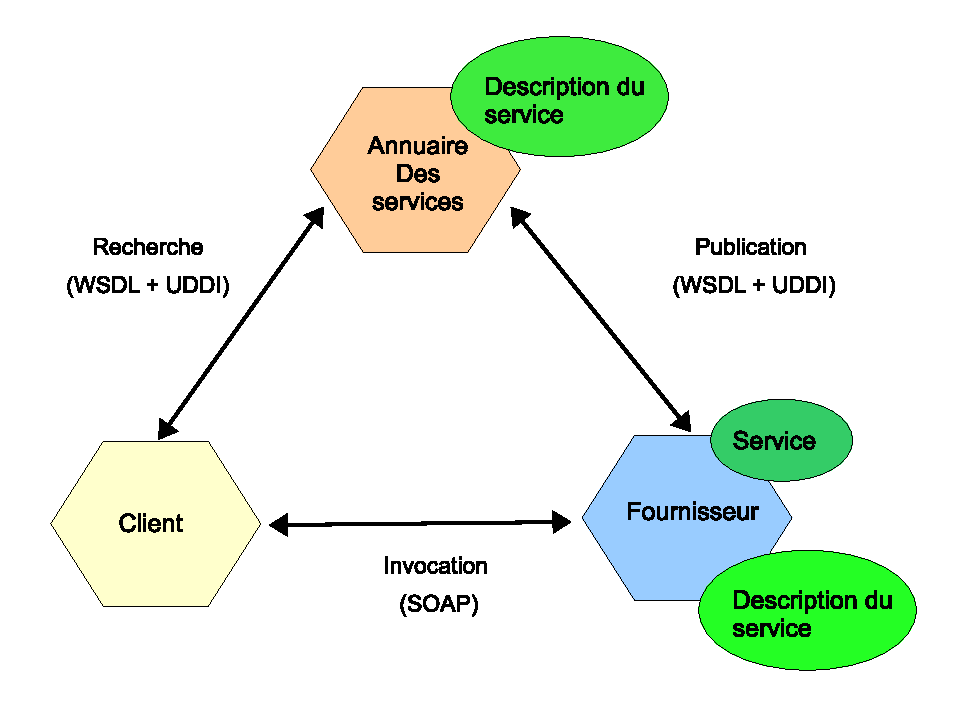
\includegraphics[width=1.1\textwidth]{figs/ws_roles.eps}
    \caption{Architecture de référence des services Web \cite{gottschalk2002introduction}}
    \label{fig:ws_roles}
\end{figure}
%%% Local Variables:
%%% mode: latex
%%% TeX-master: "../main.tex"
%%% End:

\renewcommand{\descriptionlabel}[1]{\hspace{1cm}\textbullet~\textsf{#1}}
\begin{description}
\item[Le fournisseur]: Un prestataire des services fournit l'interface
  pour le service Web et l'implémentation de l'application.

\item[L'annuaire]: Un registre de service est une façon dont les
  services Web sont officiellement publiés. Le registre de service est
  basée sur la spécification \textsc{UDDI} et reflète des informations
  sur les services fournis par le fournisseur de services.

\item[Le client]: Un client d'un service est le consommateur d'un
  service Web, il utilise le registre de service pour obtenir des
  informations et pour pouvoir accèder à un service Web.
\end{description}

Pour qu'une application profite des services Web, trois comportements
doivent avoir lieu: \textit{la publication} des descriptions du
service, \textit{la découverte} des descriptions du service et
\textit{l'invocation} des services basés sur la description du
service.

\renewcommand{\descriptionlabel}[1]{\hspace{1cm}\textbullet~\textsf{#1}}
\begin{description}
\item[Publier]: Pour être accessible, une description de service doit
  être publiée afin que le client de service puisse la
  trouver.

\item[Découvrir]: Dans l'opération de recherche, le demandeur de
  service récupère une description du service directement ou interroge
  le registre de service pour le type de service requis.

\item[Invoquer (bind)]: Finalement, un service doit être invoqué. Dans
  cette opération, le client de service invoque ou initie une
  interaction avec le service utilisant les détails de liaison dans la
  description du service pour localiser, contacter et appeler le
  service.
\end{description}

Les services Web sont construits autour de standards qui sont
\acrshort{soap}, \acrshort{wsdl} et \acrshort{uddi} assurant
respectivement leur communication, leur description et leur
découverte.

  \subsection{Communication: SOAP}
  \label{sec:soap}
  Développé par IBM\footnote{\url{http://www.ibm.com}} et
  Microsoft\footnote{\url{http://www.microsoft.com}}
  \cite{box2000simple}, Le langage \textsc{SOAP} est une
  recommandation \textsc{W3C} \cite{mitra2003soap} qui le définit
  comme étant un protocole destiné à l'échange de messages structurés,
  permettant d'invoquer des applications sur des réseaux distribués.

  \textsc{SOAP} est basé sur \textsc{XML} pour mettre en place un
  mécanisme valable d'échange des données indépendant du modèle de
  programmation de l'application et du système d'exploitation.

  Un message \textsc{SOAP} est un document XML constitué d'une
  enveloppe \textsc{SOAP} obligatoire, d'un en-tête \textsc{SOAP}
  facultatif et d'un corps \textsc{SOAP} obligatoire (voir la figure
  \ref{fig:soap-message-structure}):

  \begin{figure}[htbp]
    \centering
    \begin{subfigure}[b]{1\textwidth}        
	\centering
	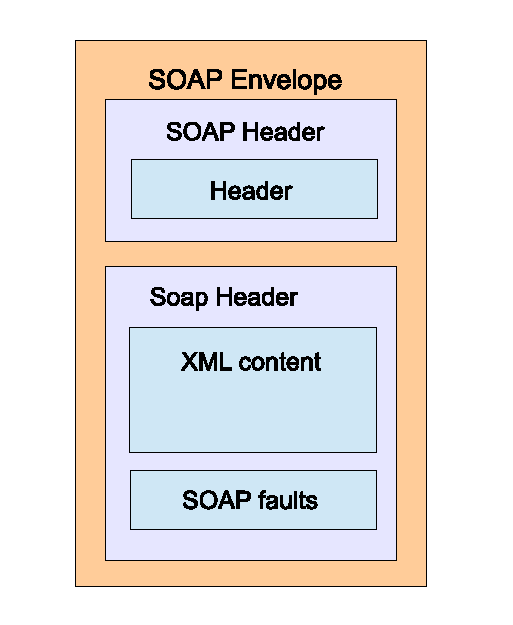
\includegraphics[width=0.5\textwidth]{figs/soap_structure.eps}
	\caption{ Les éléments d'un message \textsc{SOAP}}
	\label{fig:soap_structure}
    \end{subfigure}    

    \begin{subfigure}[b]{1\textwidth}
	\centering
	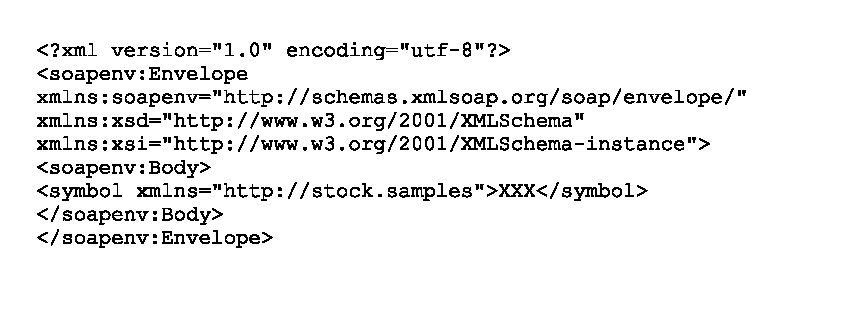
\includegraphics[width=1\textwidth]{figs/soap_message.eps}
	\caption{Exemple de message SOAP}
	\label{fig:soap-message}

    \end{subfigure}
    \caption{La structure d'un message \textsc{SOAP}}
    \label{fig:soap_all}
\end{figure}


  \renewcommand{\descriptionlabel}[1]{\hspace{1cm}\textbullet~\textsf{#1}}
  \begin{description}
  \item[Enveloppe \texttt{<Envelope>}]: L'élément racine du message
    \textsc{SOAP}, définissant le contexte du message, son
    destinataire et son contenu, il englobe l'en-tête et le corps.

  \item[En-tête \texttt{<Header>}]: Un mécanisme générique permettant
    d'ajouter des fonctions à un message \textsc{SOAP} d'une manière
    modulaire sans accord préalable entre les parties en
    communication.  Des exemples d'extension qui peuvent être
    implémentées comme des en-têtes sont des authentifications, des
    transactions, des paiements

  \item[Corps \texttt{<Body>}]: Contient les informations obligatoires
    destinées à l'ultime destinataire du message, il sert comme un
    container pour les informations mandataires à l'intention du
    récepteur du message. \textsc{SOAP} définit un élément pour le
    corps, qui est l'élément \texttt{<Fault>} (Erreur) utilisé pour
    rapporter les erreurs.
  \end{description}

  \subsection{Description: WSDL}
  \label{sec:wsdl}
  Le langage de description des services Web \acrshort{wsdl}
  \cite{christensen2001web, chinnici2007web} est une recommandation du
  \acrshort{w3c}, maintenant dans sa deuxième version.  \textsc{WSDL}
  est basé sur \textsc{XML} pour décrire les fonctions opérationnelles
  de services Web. La description \textsc{WSDL} est composée d'un
  interface et des implémentations. L'interface est une définition
  abstraite et réutilisable service qui peut être référencée par
  plusieurs implémentations.

  \begin{figure}[h]
    \centering
    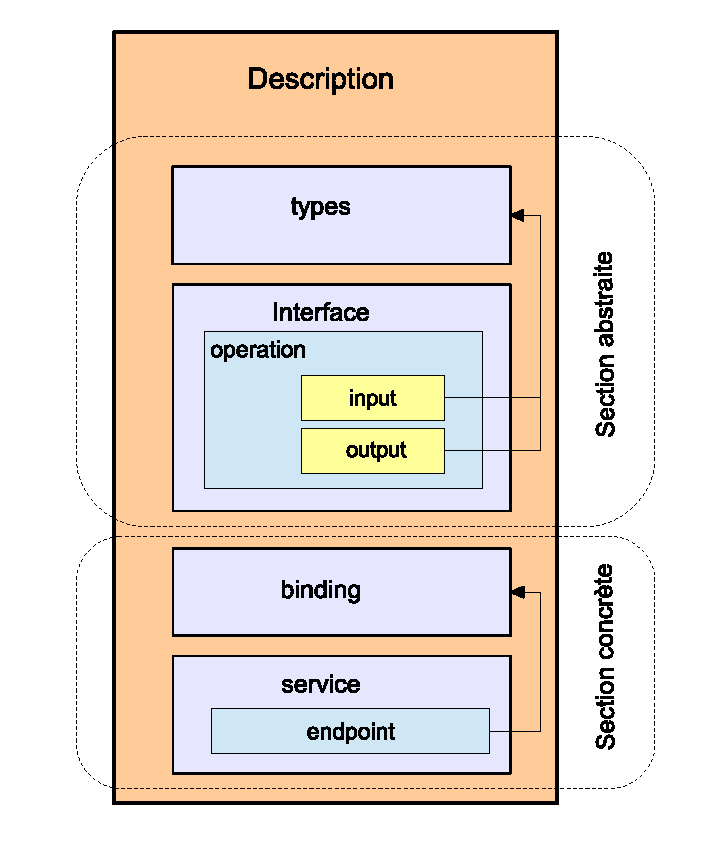
\includegraphics[width=0.6\textwidth]{figs/wsdl-document-structure.eps}
    \caption{Structure d'un message \textsc{WSDL}}
    \label{fig:wsdl-document-structure}
\end{figure}

%%% Local Variables:
%%% mode: latex
%%% TeX-master: "../main"
%%% End:


  Le langage de description de services Web \acrshort{wsdl}
  \cite{chinnici2007web} fournit un modèle ainsi qu'un langage basé
  sur \textsc{XML} de description de services Web. Un fichier
  \textsc{WSDL} comprend une description des fonctionnalités d'un
  service, mais il ne se préoccupe pas de l'implantation de celles-ci.
  Il contient aussi des informations concernant la localisation du
  service, ainsi que les données et les protocoles à utiliser pour
  l'invoquer. En pratique, le document \textsc{WSDL}
  \footnote{\url{http://www.w3.org/TR/wsdl20/}} est un document
  \textsc{XML} qui se divise en deux parties \cite{elie2010} :

  \SpecialItem
  \begin{itemize}
  \item La définition \textbf{abstraite} de l'interface du service
    avec les opérations supportées par le service Web, ainsi que leurs
    paramètres et les types des données.

  \item La définition \textbf{concrète} de l'accès au service avec la
    localisation, par une adresse réseau du fournisseur de service
    \footnote{Service Endpoint}, et les protocoles spécifiques
    d'accès.
  \end{itemize}

  La partie abstraite d'un document \textsc{WSDL} contient deux
  sous-parties:

  \SpecialItem
  \renewcommand{\descriptionlabel}[1]{\hspace{1.5cm}\texttt{#1}}
  \begin{description}
  \item[<Types>]: décrit sous la forme d'un schéma \textsc{XML} les
    types des données échangées entre le client et le fournisseur de
    services \cite{part20012}.

  \item[<Interface>]: Les interfaces\textsc{WDSL} offrent une manière
    abstraite de décrire la fonctionnalité du service, ils ont défini
    les opérations (éléments \texttt{<operation>}) en terme de
    paramètres d'entrée et de sortie sous frorme d'un un modèle
    d'échange de message \textit{(message exchange
      pattern)}. \textsc{WSDL} contient huit modèles de messages
    prédéfinis, mais on peut facilement définir de nouveaux.
  \end{description}

  La définition concrète d'un document \textsc{WSDL} est constituée
  de:

  \SpecialItem
  \renewcommand{\descriptionlabel}[1]{\hspace{1.5cm}\texttt{#1}}
  \begin{description}
  \item[<Binding>]: L'élément \texttt{Binding} reprend les opérations
    de l'élément \texttt{<Interface>} et leurs associe un protocole de
    transfert et des spécifications des formats de données de message.

  \item[<Service>]: Cet élément définit la localisation du service Web
    décrit. Pour chaque interface décrite, un élément service lui est
    associé. Le sous-élément \texttt{<endpoint>} définit un port
    d’accès en référençant l'élément \texttt{<binding>} associé et en
    déclarant l'\textsc{URL} localisant le service (avec l'attribut
    \texttt{<address>}).
  \end{description}
  % TODO: talk how WSDL description is limited, ref to the description
  % section
  \newpage
  \subsection{Découverte: UDDI}
  \label{sec:uddi}
  %TODO
  \acrshort{uddi} \cite{clement2004uddi} est une standardisation pour
  la publication et la découverte des services Web initialement conçue
  et spécifiée par le Consortium de standards
  OASIS\footnote{\url{https://www.oasis-open.org}}, il est le résultat
  d'un accord d'un ensemble d'industriels
  Ariba\footnote{\url{http://www.ariba.com/}}, IBM, Microsoft, etc en
  vue de devenir le registre standard de la technologie des services
  Web.

  \textsc{UDDI} complète les technologies basiques de services Web en
  permettant de créer un \textbf{annuaire} permettant de localiser sur
  le réseau le services web recherchés, les services référencés dans
  \textsc{UDDI} sont accessibles par l'intermédiaire du protocole de
  communication \textsc{SOAP}, et la publication des informations
  concernant les fournisseurs et les services doit être spécifiée en
  \textsc{XML} afin que la recherche et l'utilisation soient faites de
  manière \textbf{dynamique} et \textbf{automatique}.

  Un \textsc{UDDI} peut appartenir à un domaine public comme internet
  ou tout autre réseau accessible à un nombre non limité
  d'utilisateurs, comme il peut appartenir à un domaine restreint
  comme l'intranet d'une entreprise ou d'un groupe d'entreprise.

  Les données stockés dans l'\textsc{UDDI} sont structurées (en
  \textsc{XML}) et organisées en trois parties connues:

  \SpecialItem
  \begin{description}
    \item[Pages blanches]: fournissent des descriptions générales sur
      les fournisseurs de services à savoir le nom de l'entreprise qui
      fournit le service, son identificateur commercial, ses adresses,
      etc.

    \item[Pages jaunes]: comportent des descriptions détaillées sur
      les fournisseurs de services catalogués dans les pages blanches
      d'une de façon taxonomique (selon secteurs d'activités par
      exemple).

    \item[Pages vertes]: fournissent des informations techniques sur
      les services Web catalogués. Ces informations incluent la
      description du service, les adresses \textsc{URL}, du processus
      de son utilisation et des protocoles utilisés pour son
      invocation.
  \end{description}

  % TODO: talk about OWL-S and why UDDI approach is semantically poor
  % TODO : Conclure cette subsection par la mention du problème de la
  % découverte automatique des services Web et l'insuffisance de la
  % description syntaxique.
  % \newpage

\section{Description des services web}
\label{sec:ws-description}

Un service Web consiste à la définition d'une entité logiciel
modulaire, \textit{auto-descriptive} et \textit{autonome}
\textit{accessible} via Internet \cite{curbera2001web}. Dans la
section précédente, nous avons vu l'architecture de base des services
Web et la pile protocolaire pour la mise en place d'une telle
architecture.

%!TEX root = ../main.tex
\begin{figure}[h]
    \centering
    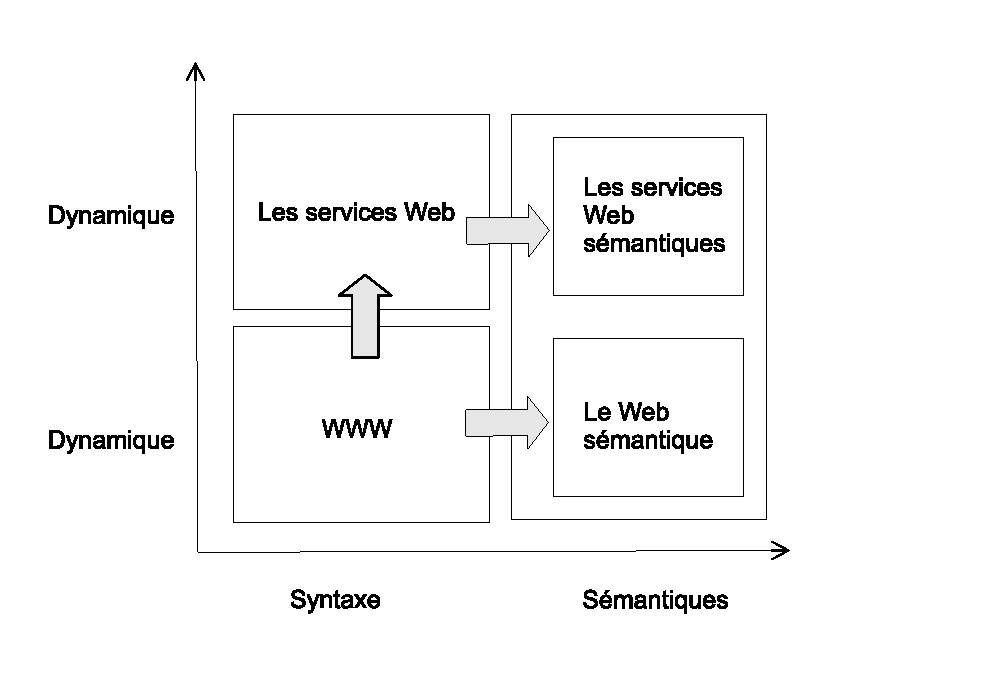
\includegraphics[width=1\textwidth]{figs/3w_to_sws.eps}
    %TODO translate
    \caption{Web evolution to Semantic Web services \cite{fensel2002semantic}.}
    \label{fig:3w_to_sws}
\end{figure}

Une description du service Web est un document par lequel le
fournisseur de services communique au client les spécifications pour
invoquer le service Web \cite{lopez2008selection}. Malgré les
améliorations apportées au standard \textsc{WSDL} dans son deuxième
version \cite{chinnici2007web}, la description du service reste
uniquement au niveau fonctionnel, c'est-à-dire qu'elle contient la
manière dont on peut utiliser le service et non ce que fait le
service, le standard \textsc{WSDL} est limité à l'énumération des
opérations et à la description des types des paramètres d'entrée et de
sortie associés, elle ne caractérise pas la sémantique de la
fonctionnalité accomplie par le service

Par conséquent, la description \textsc{WSDL} reste insuffisante lors
des processus de sélection, découvert et de la composition. Pour
pallier cette Difficulté, plusieurs approches
\cite{sivashanmugam2003adding,mcilraith2001semantic,
  mcilraith2003bringing, fensel2002web} proposent de rajouter une
couche sémantique au dessus de \textsc{WSDL} complétant la description
syntaxique par des précisions sémantiques.

% Dans cette section nous allons présenter les divers approches
% sémantiques visant à préciser la description d'un service en insistant
% sur les approches d'annotation sémantique et sur les ontologies de
% services.

Les services Web enrichis par des métadonnées supplémentaires
exprimant leur la sémantique sont appelés \textit{les services Web
  sémantiques} \cite{fensel2002semantic, mcilraith2001semantic}. Les
services de Web sémantique sont le résultat de l'évolution Web dans
deux directions \cite{bartalos2011effective} (illustré dans La figure
\ref{fig:3w_to_sws}):

\begin{enumerate}
  \item l'ajout des dynamique éléments sur le Web.
  \item l'amélioration de la description syntaxique services Web
\end{enumerate}

 La notion du Web sémantique est abordée brièvement dans l'annexe
 \ref{annexe:semantic-web}.

  \subsection{Annotations sémantiques}
  \label{sec:semantic-annot}

  L'annotation sémantique consiste à enrichir et à compléter la
  description d'un service. Elle établit des correspondances entre des
  éléments de la description et des concepts d'un ensemble
  d'ontologies de références. Une ontologie de référence permet de
  représenter un domaine par des structures interprétables par une
  machine. Deux modèles principaux suivent l'approche d'annotation
  sémantique, à savoir \textsc{WSDL-S} et \textsc{SAWSDL}
  \cite{elie2010}.

    \subsubsection{WSDL-S}
    \textsc{WSDL-S} \cite{akkiraju2005web} est le résultat d'un
    travail collaboratif entre IBM, laboratoire LSDSI et l'iniversité
    de Geogia \footnote{\url{http://www.uga.edu/}}.  La spécification
    a devenue une recommandation \textsc{W3C} depuis 2005. Son
    objectif principal est de fournir un processus d'annotation
    sémantique compatible avec les technologies
    existantes. Pratiquement, Le méta-modèle \textsc{WSDL-S} repose
    sur les capabilités du modèle \textsc{WSDL} en rajoutant trois
    éléments majeurs \texttt{<category>}, \texttt{<effect>} et deux
    attributs \texttt{modelReference} et \texttt{schemaMapping}. Les
    éléments introduits permettent de rajouter des informations qui
    n'étaient pas prises en compte dans \textsc{WSDL} comme \emph{les
      préconditions} et \emph{les effets} d'une opération. Tandis que
    les attributs permettent de référencer des concepts dans des
    ontologies de référence, ces préconditions et effets ensemble avec
    les annotations sémantiques des éléments \texttt{<inputs>} et
    \texttt{<outputs>} permet de l'automatisation du processus de
    découvert de services.

    \subsubsection{SAWSDL}
    La spécification \acrshort{sawsdl} \cite{kopecky2007sawsdl} est la
    suite de \textsc{WSDL-S} et il partage les mêmes principes de ce
    dernier. issue d'initiative du groupe de travail d'annotations
    sémantiques pour \textsc{WSDL}
    \footnote{\url{http://www.w3.org/TR/sawsdl/}} et soumise au
    \textsc{W3C} en 2007, \textsc{SAWSDL} définit un mécanisme
    d'annoter sémantiquement les interfaces et les opérations
    \textsc{WSDL}, ainsi que les types \textsc{XML schema} en les
    reliant à des concepts dans une ontologie. Cette annotation repose
    sur la définition d'attributs étendant le standard de
    description. Les annotations sémantiques référencent des
    ontologies pré-existantes. Le mécanisme d'annotation de
    \textsc{SAWSDL} est indépendant de tout langage de représentation
    \cite{lopez2008selection} d'ontologies.

    \textsc{SAWSDL} propose deux sortes d'annotations sémantiques: une
    pour identifier le concept sémantique (représentée par l'attribut
    \texttt{modelReference}) et une autre pour faire le lien entre le
    concept et le document \textsc{WSDL} (représentée par les
    attributs \texttt{liftingSchemaMapping} et
    \texttt{loweringSchemaMapping}).

  \subsection{Ontologies de services}
  \label{sec:ont-serices}

  Une ontologie de services saisit les différents aspects liés à la
  description des services et leur utilisation à travers un ensemble
  de concepts, de propriétés et de relations entre eux. Deux modèles
  d'ontologies de services sont décrits dans cette sous-section
  \textsc{OWL-S} et \textsc{WSMO} \cite{elie2010}.

    \subsubsection{WSMO}
    \label{sec:wsmo}

    \acrshort{wsmo} \cite{de2005web} est une modèle conceptuel basé
    sur la spécification \acrshort{wsmf} \cite{fensel2002web} (voir
    \ref{sec:wsmf}) pour la description des divers aspects liés aux
    services Web sémantique. Le but de \textsc{WSMO} est d'automatiser
    le cycle de vie des services web (publication, sélection,
    découverte, composition, etc.) afin de résoudre le problème de
    l'intégration des services Web en définissant une technologie
    cohérente pour description des services Web sémantique.

    Pour formaliser \textsc{WSMO}, le groupe de travail mis au point
    le langage de modélisation \acrshort{wsml} \cite{de2006web} et a
    défini plusieurs variantes de celui-ci, chacun basé sur différents
    formalismes.

    \textsc{WSMO} est constitué de quatre composants: les services
    web, les buts, les ontologies et les médiateurs. Ce modèle permet
    de réaliser un couplage faible entre les services web en utilisant
    un ensemble de médiateurs. Ces derniers assurent les tâches
    d‘intégration d'ontologies, de découverte des services, de
    composition, etc.

    \subsubsection{OWL-S}
    \label{sec:owl-s-1}
  \newpage

\section{Découverte des services web}

La découverte des services Web dans est abordée dans un grand nombre
de projets et travaux de recherche \cite{elie2010}, plusieurs
définitions sont attribuées à ce concept. Booth \textit{el al.}
décrivent le processus de découverte comme étant \textit{``la
  localisation d'une description compréhensible par la machine d'un
  service éventuellement inconnu au préalable et correspondant à
  certains critères fonctionnels''} \cite{booth2004web}. Á l'instar de
booth \cite{booth2004web}, Ankolekar \textit{el el.} ont défini la
découverte comme étant l'acte de \textit{``localiser les services Web
  (généralement par le biais d'un annuaire des services) fournissant
  un service particulier et qui adhèrent aux contraintes spécifiées''}
\cite{ankolekar2002daml}.

Ces définitions mettent l'accent sur le mécanisme de comparaison de la
requête avec les services, ainsi que son degré d'automatisation. Selon
notre point de vue la découverte de services vise à comparer une
requête d'un utilisateur avec les capacités d'un service web, et trie
les résultats selon un certain mécanisme.

Les capacités peuvent être fonctionnelles (les descriptions
d'interfaces : syntaxiques ou sémantiques, les descriptions
comportementales) ou non fonctionnelles (la qualité de service).

Plusieurs critères peuvent être utilisés pour catégoriser les
approches de découverte \cite{elie2010}, nous avons :

\begin{itemize}
\item le critère de centralisation/distribution des annuaires.
\item le principe de l'algorithme de matching (syntaxique, sémantique
  (logique, non logique), hybride, comportemental, non fonctionnel, etc.).
\item Le critère d'automatisation.
\end{itemize}

  \subsection{Localisation de services}
  \label{sec:ws-localisation}

  La découverte de services consiste, en premier, à localiser les
  fournisseurs proposant des services répondant à une requête
  utilisateur. Les approches de localisation de services récurrentes
  dans la littérature sont classées en deux catégories, à savoir les
  approches centralisées et les approches distribuées \cite{elie2010}.

  Le modèle \acrshort{uddi} \cite{clement2004uddi} (présenté dans
  \ref{sec:uddi}) dans ces premières version repose sur une approche
  \textit{centralisée} de publication et découverte de services
  Web. \textsc{UDDI} définit un modèle de représentation des données
  et des méta-données nécessaires à la publication, reposent sur
  \textit{un seul annuaire} qui peut être géré par un module de mise
  en correspondances \textit{(matchmaker)}.

  Les approches distribuées de découverte de services consistent à
  mettre en place une communauté (fédération) d'annuaires
  \textsc{UDDI} \cite{rompothong2003query,
    sivashanmugam2004discovery}.

  Dans \cite{sivashanmugam2004discovery}, les auteurs proposent de
  fournir un service qui agit comme une couche d'abstraction reliant
  plusieurs instances \textsc{UDDI}. Chaque instance de \textsc{UDDI}
  est responsable des données concernant les services auxquels elle
  fait référence.

  Dans \cite{verma2005meteor}, les auteurs présentent
  \textsc{METEOR-S}, une infrastructure pair-à-pair extensible,
  d'annuaires pour la publication de services Web sémantiques et leur
  découverte permettant la collaboration entre plusieurs instances
  d'annuaires \textsc{UDDI}.

  La dernière version d' \textsc{UDDI} \cite{oasis2005specification}
  (version 3.0.2) reprend le principe d'une fédération
  d'annuaires. Elle décrit un annuaire \textsc{UDDI} comme un ensemble
  de nœuds \textit{(UDDI nodes)} tel que chaque nœud fait partie d'un
  seul annuaire et possède une copie répliquée de schéma globale de la
  fédération. Les nœuds d'un annuaire collaborent pour gérer un
  ensemble de structures de données \textsc{UDDI} et permettre une
  meilleure gestion des requêtes.

  \subsection{Découverte manuel/automatique}
  \label{sec:ws-desc:manual-vs-auto}
  \newpage

  \subsection{Matching des services Web}
  \label{sec:ws-matching} Le processus de matchmaking repose sur la
  recherche de similarités entre les paramètres descriptives de ces
  derniers. Il existe deux catégories de paramètres de description des
  services web: les paramètres fonctionnels et les paramètres
  non-fonctionnels que nous décrivons tout de suite.

    \subsubsection{Paramètres de description des services web}
    \label{sec:param-de-descr}

    \SpecialItem
    \begin{description}
    \item [Le coût]: C’est une propriété non-fonctionnelle qui est
      pertinente pour le client qui veut utiliser le service.

    \item [La sécurité]: La sécurité est une propriété
      non-fonctionnelle qui est pertinente à la plupart des services
      web. Elle applique des aspects tels que la communication et le
      cryptage des données.

    \item [La qualité]: La propriété qualité des services est un
      ensemble de propriétés différentes qui affecte tous les aspects
      spécifiques du service, son utilisation et sa production tel que
      le temps de réponse d'un appel à une opération, la capacité du
      service...etc
    \end{description}

    \subsubsection{Le modèle syntaxique de matching des services Web}
    \label{sec:syntactic-matching}

    \subsubsection{Le modèle sémantique de matching des services Web}
    \label{sec:semantic-matching}

\newpage
\section{Conclusion}
% faire un petit récapitulatif sur les technologies des services web
% rappeler de notre problème principale : composition des services web

%%% Local Variables:
%%% mode: latex
%%% TeX-master: "../main"
%%% End:
